%\documentclass[12pt]{amsart}
\documentclass[12pt,notitlepage]{article}

\usepackage{geometry}                % See geometry.pdf to learn the layout options. There are lots.
\geometry{a4paper}                   % ... or a4paper or a5paper or ... 
%\geometry{landscape}                % Activate for for rotated page geometry
%\usepackage[parfill]{parskip}    % Activate to begin paragraphs with an empty line rather than an indent
\usepackage{graphicx}
\usepackage{amssymb}
\usepackage{epstopdf}
\usepackage{hyperref}
\usepackage{datetime}
%
\DeclareGraphicsRule{.tif}{png}{.png}{`convert #1 `dirname #1`/`basename #1 .tif`.png}

\title{Analysis of the San Francisco Crime Classification problem, from ``kaggle.com"}
\author{Stephen R. Williams}
\date{\today}                                           % Activate to display a given date or no date

\begin{document}
\maketitle

\begin{abstract}
Here I explain the problem and document my efforts in competing in the \emph{kaggle} competition for \emph{San Francisco Crime Classification}. The problem aspires towards the optimal prediction for the likelihood for each of 39 possible crime categories having occurred, given a training data set and measured against a the test data set. The test data types can be divided into two broad categories, firstly the precise time and date at which the crime was reported to police, and secondly the location where it occurred. Here I will steadily and systematically build up towards my chosen approach. This approach is a variation on a \emph{naive Bayes} method, with the time and location being treated as independent of each other. In addition I predict the time dependent behaviour by using a Fourier decomposition on the training data. The spatial data analysis will employ a basic approach, combined with data feature engineering. \emph{Python} is the main tool used throughout this project.
\end{abstract}

\section{Introduction (\emph{The Problem})}

The competition may be found at \url{https://www.kaggle.com/c/sf-crime} The problem consists of crime reports to police in San Francisco over the period 6/01/2006 through to 10/05/2005 with alternating weeks divided between the \emph{test data set} and the \emph{training data set}. The data set has the following data categories (with some only in the training set (noted as: train.csv)),

\begin{itemize}
\item Dates - timestamp of the crime incident
\item Category - category of the crime incident (only in train.csv). This is the target variable you are going to predict.
\item Descript - detailed description of the crime incident (only in train.csv)
\item DayOfWeek - the day of the week
\item PdDistrict - name of the Police Department District
\item Resolution - how the crime incident was resolved (only in train.csv)
\item Address - the approximate street address of the crime incident 
\item X - Longitude
\item Y - Latitude,
\end{itemize}
%
and we are required to predict the Category for the test set. There is not enough information available to predict the particular crime category with any reliability, and the idea is to predict the likelihood of each 39 possible category outcomes. This is forced upon us by the way our entries are scored, using a \emph{multi-class logarithmic loss} formula
%
\begin{equation}
logloss = -\frac{1}{N}\sum_{i=1}^N \sum_{j=1}^M y_{ij} \ln(p_{ij}),\label{eq:logloss}
\end{equation}
%
where $N=884,262$ is the number of crime incidents in the test set, $M=39$ is the number of possible crime category outcomes, $y_{ij}$ is unity if the actual (not known to us) crime category for incident $i$ happens to coincide with category $j$ and zero otherwise, and $p_{ij}$ is the probability we have predicted for category $j$ being the actual (not known to us) crime category reported for incident $i$. Given a suitable mathematical background, it is easy to see that this $logloss$ quantity has the property that the absolute statistical errors in our predictions for each of the 39 categories are of equal importance. That is the absolute error in our prediction for the probability of a very unlikely outcome is of equal importance to the absolute error in our prediction for a very likely outcome. However one should realise that if we correctly identify an outcome as being very unlikely, then it's absolute error will be correspondingly very small. Let us start by making a submission that makes use of this observation, and very little more.

\section{Trial 1: An entropic approach}
Given Eq. (\ref{eq:logloss}) let us consider the optimal way of scoring upon ignoring all information based on time and space. That is, if we submit the same 39 probabilities for all of the $N=884,262$ crime incidents, what is the optimal probability weightings. In the limit where $N\rightarrow \infty$ this score will be given by the entropy
%
\begin{equation}
S = -\frac{1}{39}\sum_{j=1}^{39} p_j \ln{p_j},
\end{equation}
where $p_j$ is the global probability for the $j_{th}$ crime category occurring, and in this limit the global probabilities will correspond to the optimal probability weightings. I will not go into the details of how and why this is the case, just hope you accept my assertion of it being so. With this in mind let us compute the global probabilities for each of the 39 crime categories, using the training data, then compute the entropy, and see what happens upon making a \emph{kaggle} submission. But first lets see what these global probabilities look like.
%
\begin{figure}
\centering{}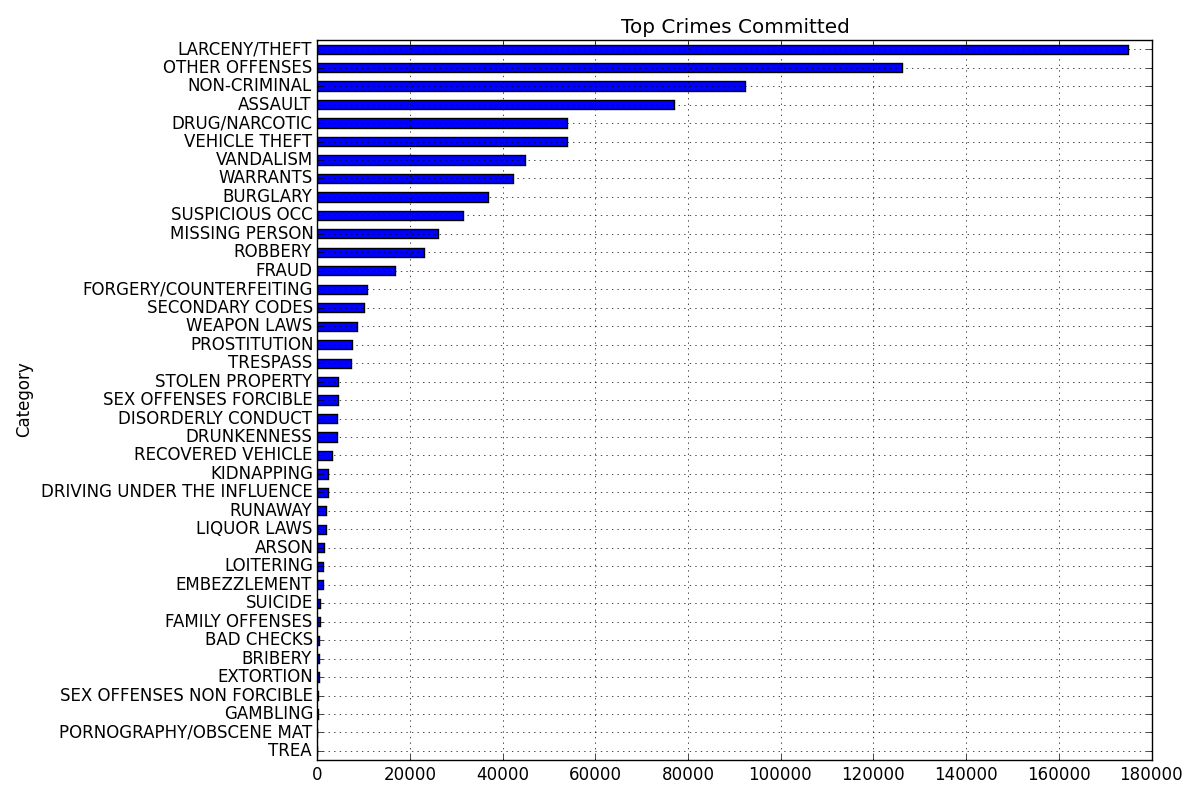
\includegraphics[scale=0.4]{crime-histo}\caption{ Histogram of crime categories, ranked from most to least prevalent \label{fig:crime-hist}}
\end{figure}
%
There are some good graphing scripts that have been put up by the community on the \emph{kaggle} site. I have slightly modified one of these to make a histogram of the various crime categories ordered by their prevalence. The \emph{Python} script is here in my GitHub repository as entropy\textbackslash crime-graphs.py and the relevant graph can be seen in Fig. (). On average there are $884,262 / 39 \simeq 22,700$ per category, and from the graph we see that the top crime category of LARCENY/THEFT is around 8 times more likely than the average, the twelfth most prevelent crime of ROBBERY is close to the average value, and by the time we are half way through the list of categories (say STOLEN PROPERTY) we are down to a frequency that is approximately 5 times less than the average. The most prominent quarter to a third of categories contain the vast majority of occurrences.  
%\section{}
%\subsection{}

\end{document}  